\section{The project structure}

The code we developed consists of 5 files (excluding the wrappers, described in the previous section). They are \texttt{train.py}, \texttt{pre_encode.py}, \texttt{infere_plain.py}, \texttt{infere_enc.py} and \texttt{post_decode.py}. The scripts must be executed one at a time, in a particular order, because they are interdependent: they produce output tensors which are then used by the scripts in the subsequent phases. The tensors are saved in the \texttt{nn_data} and \texttt{output_data} folders. The dataflow is enclosed in the following diagram:

\begin{figure}[H]
	\centering
	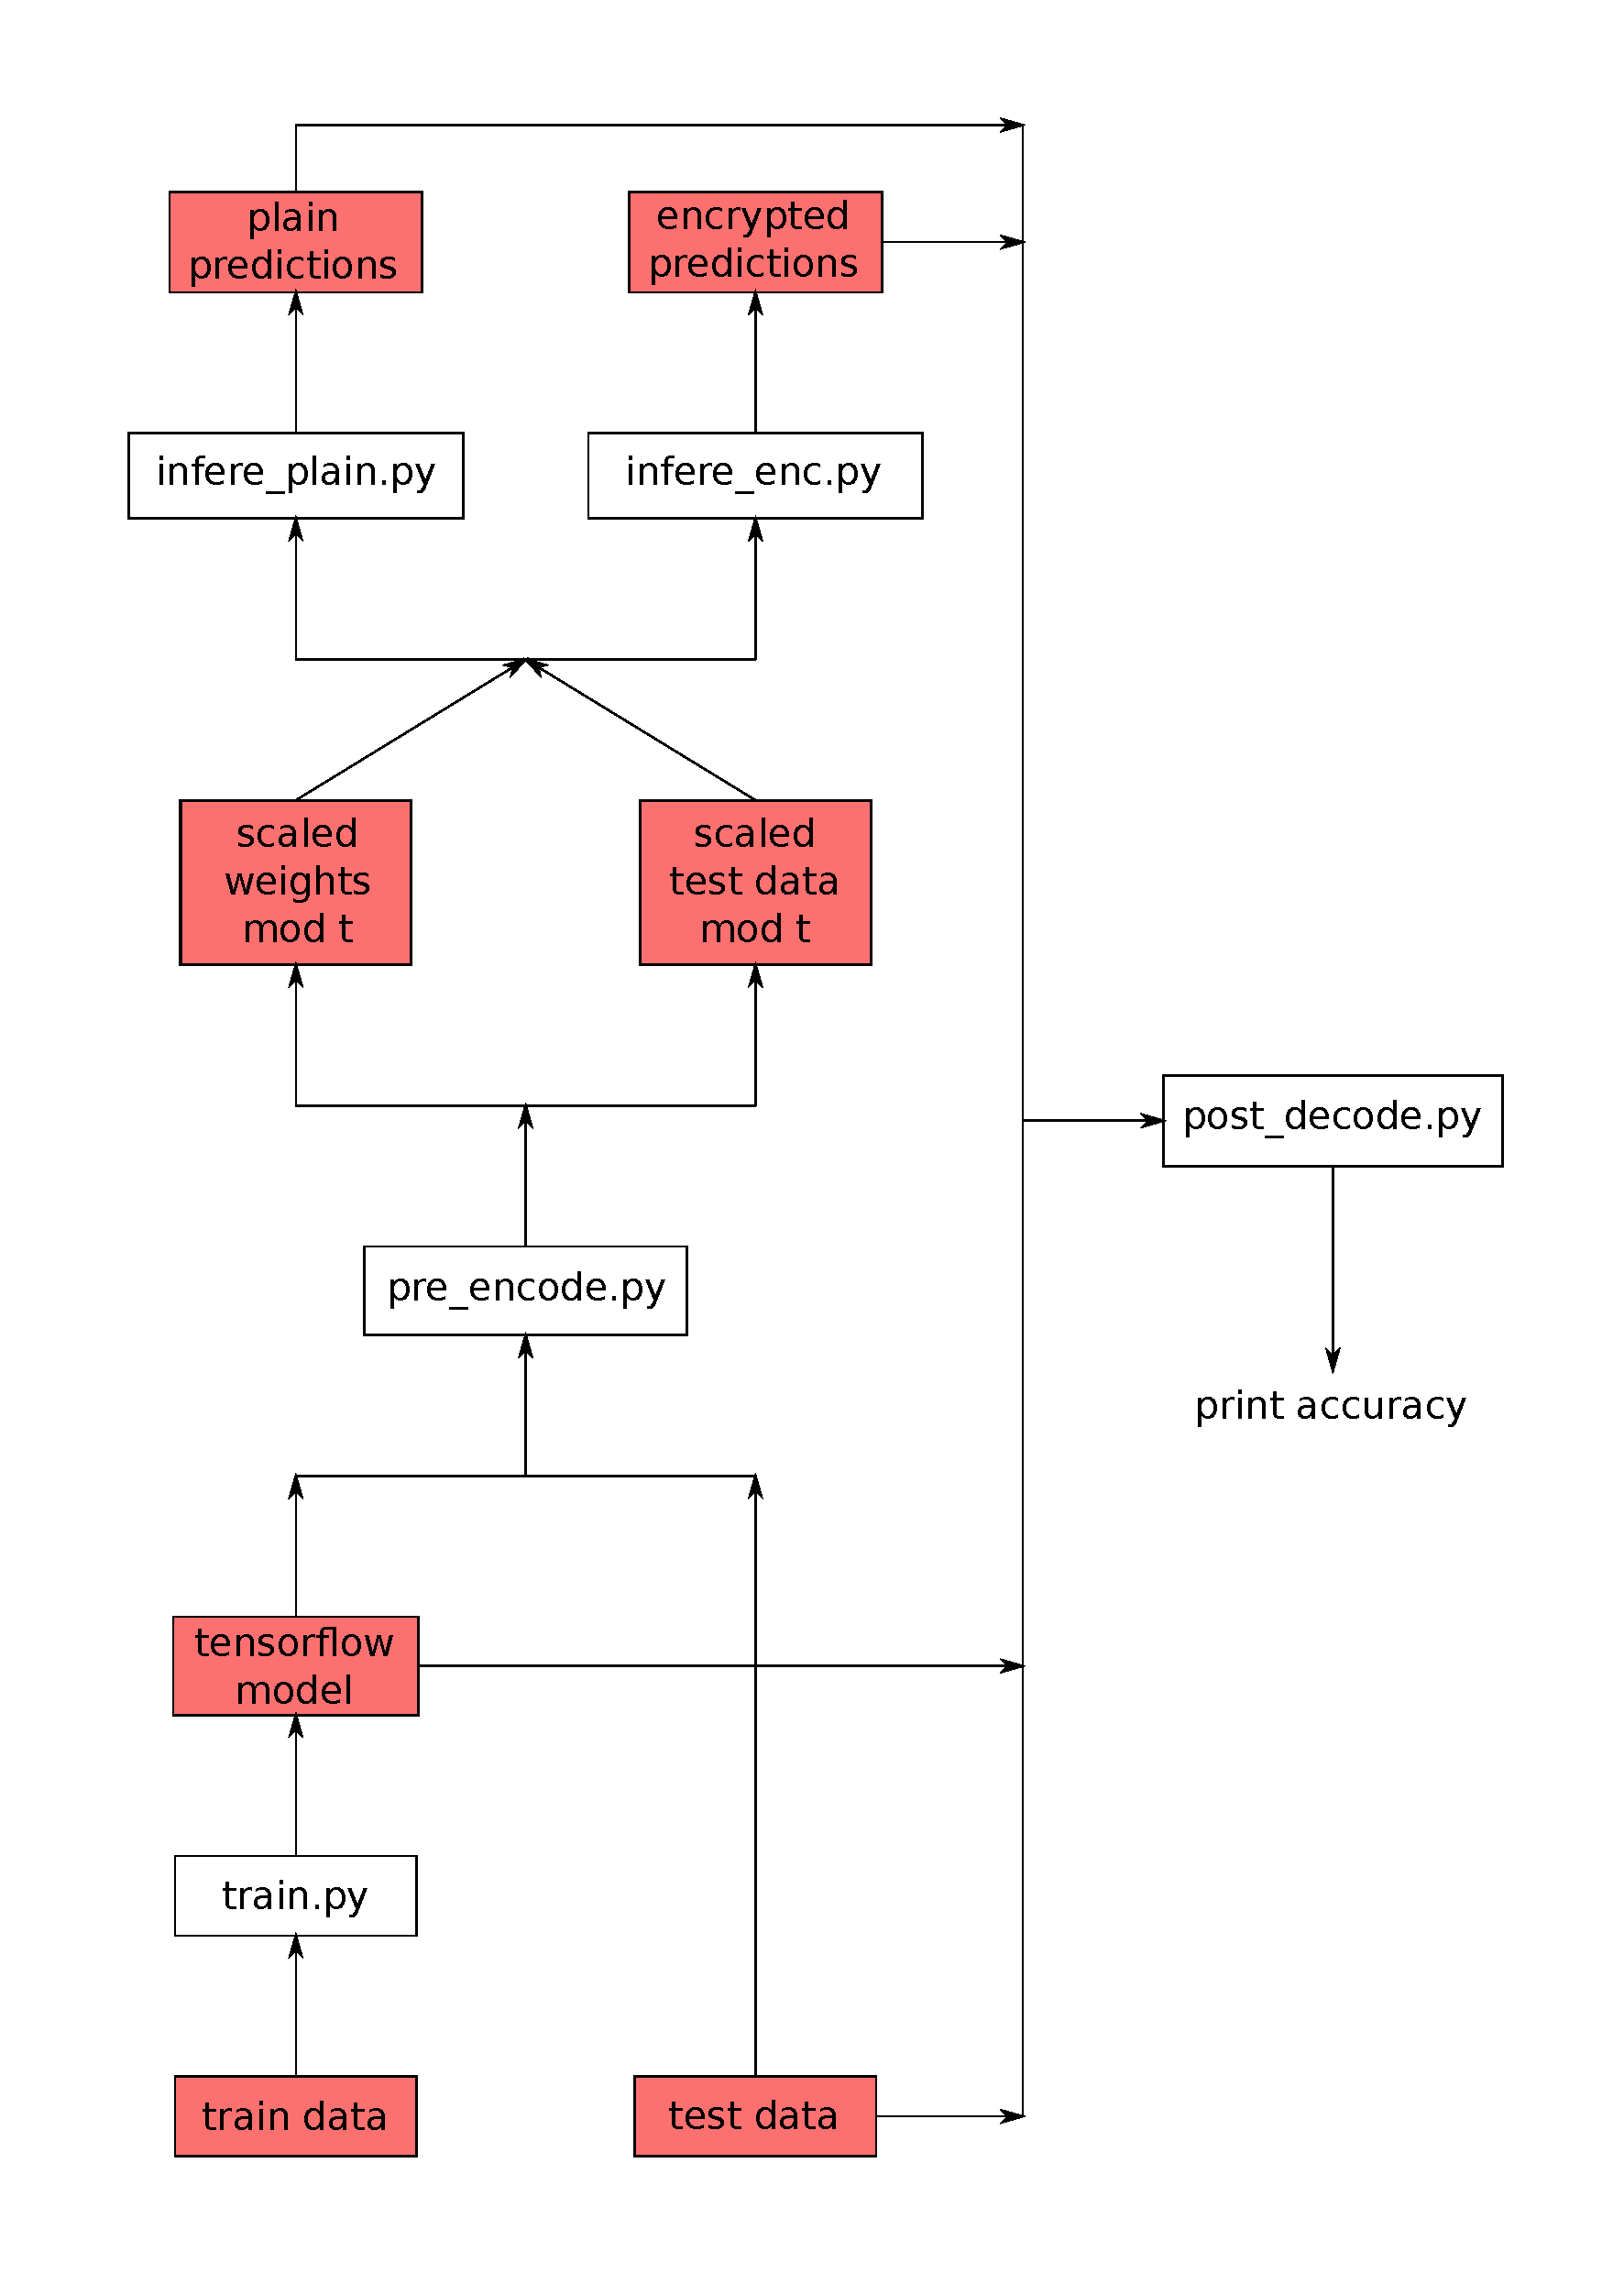
\includegraphics[width=0.9\textwidth]{images/fig4a.pdf}
    \caption{The flow scheme of data between the scripts.}
    \label{fig:im4}
\end{figure}

\subsection{\texttt{train.py}}

As you can see from the diagram, the first script to be executed is \texttt{train.py}. It uses 55000 images and labels from the MNIST database to train a neural network, thanks to the TensorFlow library. The only operations used are sum and product. The network is described in detail in the Section 3: Neural network.

\subsection{\texttt{pre_encode.py}}

When executed, this file loads in memory the TensorFlow model generated by \texttt{train.py} from the \texttt{nn_data} folder and applies, on the model as well as on the dataset test, the pre-encoding phase: it multiplies each value by a constant called precision, and performs the reduction modulo $t_i$, with $i = 0,1,2,3,4$. Thus obtains 5 numbers in output for each input number, ie five times the size of the input tensor. The image data and the weights of the neural network thus obtained are saved, respectively, in the \texttt{output_data} folder (with the name of \texttt{plain_layer_0.npy}) and in the \texttt{nn_data} folder.

\subsection{\texttt{infere_plain.py}}

Unlike the other files, \texttt{infere_plain.py} is not strictly necessary for the execution of the project. In fact it was initially developed during the testing and debugging phase of the CryptoNets, but, because it has an intermediate model between the final neural network and the base model calculated with tensorflow, it is useful in order to understand the project. After loading weights and input data into memory, the remaining part of the code is divided into 5 parts, corresponding to the 5 layers of the network. After each layer, it saves the output tensor in the \texttt{output_data} folder (this operation was very useful during the debugging phase). The first layer, the most complicated one, is the convolution layer: for each of the five filters in the map_count, it shifts the filter on the input images, performs a multiplication element-wise, and sums all the values obtained, together to the bias. The resulting sum is reduced modulo $t_i$, and the result is saved in a new output tensor. The indexes of the input and output tensors works in such a way that each image is flattened after the computation. Layers 2 and 4 are identical, and perform the element-wise square operation. Layers 3 and 5 instead correspond to two fully connected layers and take advantage of the NumPy operator .dot() to perform this calculation.

\subsection{\texttt{infere_enc.py}}

\texttt{infere_enc.py} works like \texttt{infere_plain.py}, with the difference that the input data is first encoded and then encrypted. The data are saved after the application of each layer. Moreover, they are saved two more times: once at the beginning, after the encoding and encryption phase, and once at the end, after having executed the inverse procedure. The main difference consists instead in how the input examples are managed: in \texttt{infere_plain.py} the data could and had to be managed separately, but not here. In \texttt{infere_enc.py}, since the data has been encoded in polynomial arrays, the data must be taken in blocks of $(n+1)\cdot\text{q_size}\cdot2$, ie each polynomial must be considered as a single object. Therefore, the index that ran through the images in \texttt{infere_plain.py} becomes four nested for: one to scroll through the blocks of the encrypted messages, one to scroll on the elements of each array, one to scroll on the dividers $q_i$, and one to scroll through the coefficients of each polynomial:

\lstset{frame=tb,
  language=Python,
  breaklines=true,
  showstringspaces=false,
  columns=flexible,
  numbers=left,
  commentstyle=\color{dkgreen},
  stringstyle=\color{mauve},
  tabsize=3
}
\begin{lstlisting}[frame=single]
for poly_group_index in range(poly_groups_count):
  for s_index in range(2):
    for q_index in range(q_size):
      for n_index in range(n_parm+1):
        axis0_index = n_index + (q_index*(n_parm+1)) + (s_index*q_size*(n_parm+1)) + (poly_group_index*enc_poly_size)
        ...
\end{lstlisting}

We added also a print function between lines 3 and 4 which indicates the percentage of progress made for this layer. Layers 3 and 5 work as in the case of \texttt{infere_plain.py}, ie use the NumPy .dot() operator. But in this case, the tensor dtype can no longer be np.uint64, but must be of the object type. This is due to the fact that the data in question are reduced modulo $q_i$, while the weights are reduced modulo $t_i$. This means that while the network weights can reach a maximum of 18 bits (unsigned), the input data values are at most 60 bits. During the multiplication between weights and data the values are therefore 78 bits long, before they get reduced modulo $q_i$, and so brought back into the 60 bit limit. If you force a tensor this way, NumPy automatically transforms the output dtype from np.uint64 to np.float64: the 52 bits of mantissa of the np.float64 type are therefore not enough to contain the entire 78-bit information (before it is reduced with the modulo operation), and there is therefore a loss of precision. This would not be much of a problem if we were operating in the plain data space, but since they are encrypted messages, the loss of precision prevents the FV algorithm from correctly reconstructing the output, resulting in a gibberish output. To prevent this from happening, the tensor must then be forced to use the integer type of Python; in fact it has native support for integers greater than the size of a register (64 bits). In order to accomplish this, we created a function called to_object_dtype() that does just that. After performing multiplication with the .dot() operator, we perform the reduction modulo $q_i$, and finally we add the bias multiplied by the scaling factor $k$ (and reduced again modulo $q_i$). Layers 2 and 4 perform squaring using the function inside the SEAL library.

\subsection{\texttt{post_decode.py}}

The files produced by the two types of inference (plain and encrypted) are compared to see if they are equal. If they are the same, it means that the output calculated through \texttt{infere_enc.py} is correct in the sense that it performed operations on encrypted data in the same way that operations were performed from the file \texttt{infere_plain.py}. In fact, the loss of accuracy in the transition between the model with plain integers and the model with integers but encrypted is and must be zero. The only factor that contributes to the loss of accuracy is in fact the use of integers instead of the original model with real numbers. After comparing the two input files, assuming they are equal, it reconstructs the output using the inverse operation of the crt. It calculates predictions with the argmax() function and also calculates predictions using the original model with real numbers. Finally it prints the accuracy of these two models to compare them.
